% % % % % % % % % % % % % % % % % % % % % % % % % % % % % % % % % %
%  Devolutiva — Fase 1: Imersão
%  Disciplina: Design Thinking (DE_233) — ETE Cícero Dias
%  Profa. Samara Silva  ·  Recife, 17 de junho de 2026
% % % % % % % % % % % % % % % % % % % % % % % % % % % % % % % % % %

\documentclass[
  sigconf,
  nonacm, % Remove o rodapé da ACM
  language=portuguese
]{acmart}

% ── Desliga rodapé ACM ──────────────────────────────────────
\settopmatter{printacmref=false}
\setcopyright{none}
\acmYear{2026}
\let\balance\relax

% ── Mata a página temporária da ACM (compilação única via API) ──
\makeatletter
\def\acm@addtemp@page{}
\makeatother

% ── Pacotes ─────────────────────────────────────────────────
\usepackage[portuguese]{babel}
\usepackage{microtype}
\usepackage{booktabs}
\usepackage{tabularx}
\usepackage{array}
\usepackage{colortbl}
\usepackage[dvipsnames,table]{xcolor}
\usepackage[inline]{enumitem}
\usepackage{graphicx}
\usepackage{adjustbox}
\usepackage{fancyhdr}
\usepackage{eso-pic} % Para a capa preencher toda a página sem gerar páginas em branco

% ── Ajuste contra quebras de texto ruins (Textos Cortados) ──
\tolerance=1000
\emergencystretch=1.5em

% ── Cores ───────────────────────────────────────────────────
\definecolor{cgood}{HTML}{1E6B3A}
\definecolor{cwarn}{HTML}{8B4500}
\definecolor{cred}{HTML}{C0392B}
\definecolor{cmuted}{HTML}{666666}
\definecolor{crow}{HTML}{F2EFEB}

% ── Colunas customizadas para tabela ────────────────────────
\newcolumntype{L}[1]{>{\raggedright\arraybackslash}p{#1}}
\newcolumntype{C}[1]{>{\centering\arraybackslash}p{#1}}

% ── Comando nota destacada ───────────────────────────────────
\newcommand{\notadestaque}[2]{%
  \noindent\textbf{Nota:}\enspace%
  {\large\bfseries\color{cred}#1\,/\,#2\,pts}%
}

% ── Comando label de status ──────────────────────────────────
\newcommand{\statusok}[1]{{\small\bfseries\color{cgood}#1}}
\newcommand{\statuswarn}[1]{{\small\bfseries\color{cwarn}#1}}

% ── Renomeações PT-BR ────────────────────────────────────────
\AtBeginDocument{%
  \renewcommand{\abstractname}{Resumo}
  \renewcommand{\figurename}{Figura}
  \renewcommand{\tablename}{Tabela}
}

% ────────────────────────────────────────────────────────────
\begin{document}

% ── CAPA ────────────────────────────────────────────────────
\thispagestyle{empty}
\AddToShipoutPictureBG*{%
  \AtPageLowerLeft{%
    \IfFileExists{capa-definicao.png}{%
      
\includegraphics[width=\paperwidth,height=\paperheight]{capa-definicao.png}%
    }{%
      \IfFileExists{../../capa-definicao.png}{%
        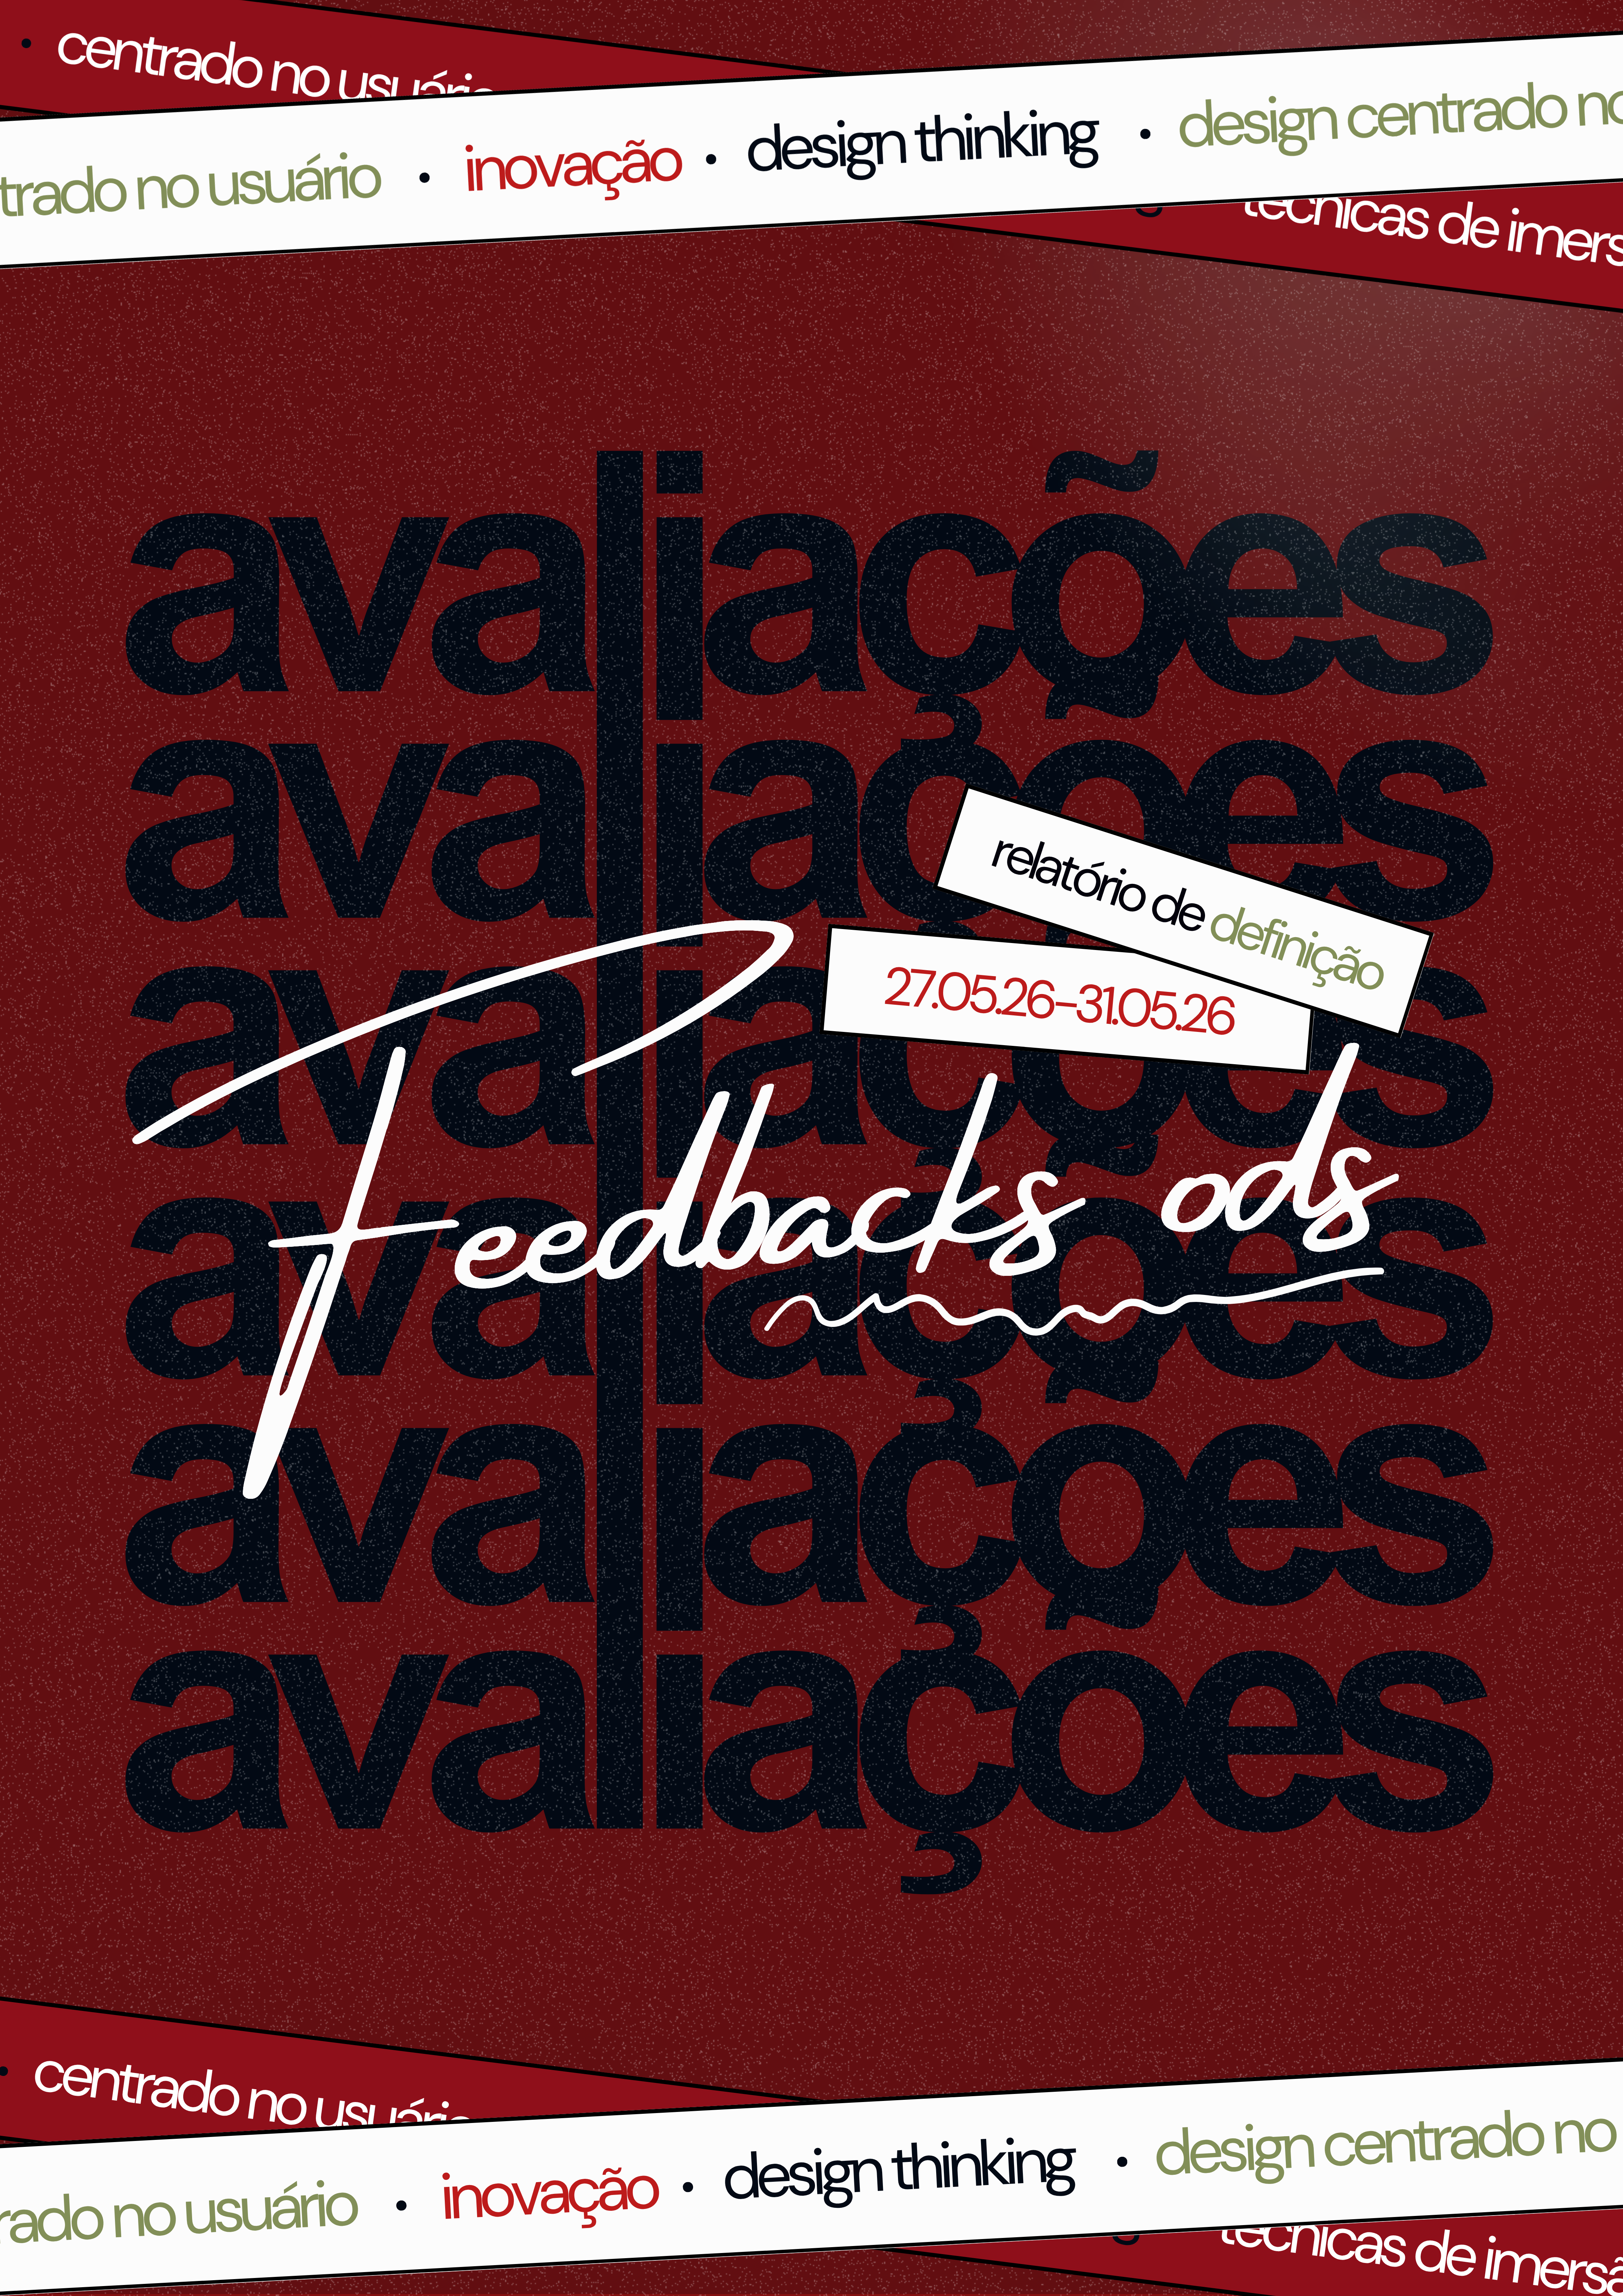
\includegraphics[width=\paperwidth,height=\paperheight]{../../capa-definicao.png}%
      }{%
        \parbox[b][\paperheight]{\paperwidth}{%
          \vspace*{10cm}\begin{center}{\large\color{gray}[capa-definicao.png não encontrada]}\end{center}%
        }%
      }%
    }%
  }%
}
\mbox{} % Caixa vazia para garantir que a página da capa seja gerada e preenchida
\clearpage

% ── CONFIGURAÇÃO DE PÁGINA PÓS-CAPA ─────────────────────────
\setcounter{page}{1}
\pagestyle{fancy}
\fancyhf{}
\renewcommand{\headrulewidth}{0pt}
\fancyfoot[C]{\thepage}
\setlength{\headsep}{0.8cm} % Distancia o cabeçalho do conteúdo das colunas

% ── METADADOS ────────────────────────────────────────────────
\title{Feedback Avaliativo de Projeto: Design Centrado no Usuário --- Fase 2 — Definição (lente DCU)}

\author{Profa.\ Samara Silva}
\authornote{Grupo: \textbf{Grupo 01 - Fome Zero} \textperiodcentered\ Per\'{i}odo: 27-31 de maio de 2026 \textperiodcentered\ Avaliado em: 17 de junho de 2026.}
\email{samarasilvia.educa@gmail.com}
\affiliation{%
  \institution{ETE C\'{i}cero Dias}
  \department{M\'{o}dulo 1 --- Turma A · 2026.1}
  \city{Recife}
  \state{Pernambuco}
  \country{Brasil}
}

\author{Grupo 01 - Fome Zero}
\affiliation{%
  \institution{ETE C\'{i}cero Dias}
  \department{Turma --- Turma A · 2026.1}
  \city{Recife}
  \state{Pernambuco}
  \country{Brasil}
}
\maketitle

\vspace{1em}
\section{Avaliação Geral}

\notadestaque{3,10}{5,00}

A avaliação foi concluída. A seguir o resumo dos critérios e os comentários detalhados.

\subsection{Resumo dos Critérios}

\rowcolors{2}{crow}{white}
\begin{tabular}{@{} L{2.6cm} C{2.5cm} C{1.1cm} C{1.1cm} @{}}
\toprule
\textbf{Critério} & \textbf{Status} & \textbf{Nota} & \textbf{Máx.} \\
\midrule
Persona — Qualidade Visual e Estrutura & \statuswarn{Completo c/ ressalvas} & \textbf{1,27} & 2,00 \\
Jornada do Usuário AS TO IS — Qualidade Visual & \statuswarn{Faltou pouco} & \textbf{0,98} & 1,50 \\
Mapa de Empatia — Apresentação Visual & \statuswarn{Completo c/ ressalvas} & \textbf{0,85} & 1,50 \\
\midrule
\textbf{Total} & & \textbf{\color{cred}3,10} & \textbf{5,00} \\
\bottomrule
\end{tabular}

\section{Comentários por Critério}

\subsection{Persona — Qualidade Visual e Estrutura}

\noindent\statuswarn{1,27\,/\,2,00 pts · Completo c/ ressalvas}

\begin{itemize}[leftmargin=14pt,itemsep=1pt,topsep=3pt,parsep=0pt]
  \item[\textcolor{cgood}{$\checkmark$}] {\small\textcolor{cgood}{A persona é visual e bem diagramada — hierarquia clara e legível}}
  \item[\textcolor{cgood}{$\checkmark$}] {\small\textcolor{cgood}{Cor e tipografia coerentes}}
  \item[\textcolor{cgood}{$\checkmark$}] {\small\textcolor{cgood}{As informações estão organizadas com clareza}}
  \item[$\square$] {\small\textcolor{cmuted}{(usabilidade) Proficiência tecnológica / letramento digital — quão à vontade a persona está com a tecnologia da solução. Sem isso não dá pra calibrar a complexidade da interface.}}
\end{itemize}

\textbf{Critérios de avaliação considerando Design Thinking e Design Centrado no Usuário }

Ao analisar os artefatos, é importante considerar duas perspectivas complementares:

\begin{itemize}[leftmargin=14pt,itemsep=2pt,topsep=4pt]
  \item \textbf{Design Thinking (DT):} foca na estrutura do processo, organização das etapas e coerência entre artefatos.
  \item \textbf{Design Centrado no Usuário (DCU):} aprofunda a compreensão do usuário real, sua experiência, limitações, contexto e interação com tecnologia.
\end{itemize}

\textit{\textbf{persona do ponto de vista de dcu}}

A persona está bem construída do ponto de vista visual e estrutural, apresentando boa hierarquia, legibilidade e coerência estética entre os elementos. A organização das informações também contribui para uma leitura clara e objetiva, além de demonstrar consistência na identidade visual do projeto.

No entanto, sob a perspectiva de Design Centrado no Usuário (DCU), observa-se a ausência de um elemento importante relacionado à usabilidade: o \texttt{letramento digital} da persona. Não há uma indicação clara sobre o nível de proficiência tecnológica do usuário, o que é essencial para calibrar adequadamente a complexidade da solução proposta.

Esse tipo de informação ajuda a compreender o quanto o usuário está habituado ao uso de tecnologias, aplicativos e interfaces digitais, além de indicar possíveis limitações ou facilidades na interação com a solução. Sem essa definição, a persona perde uma camada importante de profundidade para decisões de design.

\subsection{Jornada do Usuário AS TO IS — Qualidade Visual}

\noindent\statuswarn{0,98\,/\,1,50 pts · Faltou pouco}

\begin{itemize}[leftmargin=14pt,itemsep=1pt,topsep=3pt,parsep=0pt]
  \item[\textcolor{cgood}{$\checkmark$}] {\small\textcolor{cgood}{Apresentação visual clara com boa hierarquia}}
  \item[\textcolor{cgood}{$\checkmark$}] {\small\textcolor{cgood}{Coerência persona → solução — os objetivos e o contexto sustentam as decisões de design que o grupo tomou depois.}}
  \item[$\square$] {\small\textcolor{cmuted}{Identifica dores e oportunidades de design}}
  \item[$\square$] {\small\textcolor{cmuted}{Ferramentas/canais que usa HOJE pra lidar com o problema (WhatsApp? ligação? presencial? rádio?)}}
  \item[$\square$] {\small\textcolor{cmuted}{Pontos de atrito tecnológico (informação não chega no canal que usa? demora? não confia?)}}
  \item[\textcolor{cgood}{$\checkmark$}] {\small\textcolor{cgood}{Comportamentos de uso atuais (como ela interage com a tecnologia disponível hoje?)}}
\end{itemize}

\textit{\textbf{mapa de empatia do ponto de vista de dcu}}

A jornada do usuário apresenta uma estrutura visual clara e organizada, com boa hierarquia e coerência entre as etapas. Além disso, há consistência entre a persona, o problema identificado e a proposta geral da solução, o que demonstra alinhamento dentro do processo de Design Thinking.

Porém, em uma análise mais aprofundada sob a perspectiva do \textbf{Design Centrado no Usuário}, a jornada ainda se mostra simplificada. Faltam elementos essenciais como a identificação de \texttt{dores e oportunidades} em cada etapa da experiência, o que limitaria uma compreensão mais completa do comportamento do usuário ao longo do processo.

Também não são evidenciados com clareza os canais e ferramentas que o usuário utiliza atualmente para lidar com o problema, como WhatsApp, ligações, pesquisas online ou interações presenciais. Esse mapeamento é importante para compreender a experiência real antes da solução proposta.

Outro ponto importante é a ausência de pontos de atrito tecnológico, como dificuldades no recebimento de informações, demora em respostas ou falta de confiança em determinados canais. Esses elementos são fundamentais para identificar falhas na experiência atual e justificar oportunidades de melhoria.

\subsection{Mapa de Empatia — Apresentação Visual}

\noindent\statuswarn{0,85\,/\,1,50 pts · Completo c/ ressalvas}

\begin{itemize}[leftmargin=14pt,itemsep=1pt,topsep=3pt,parsep=0pt]
  \item[\textcolor{cgood}{$\checkmark$}] {\small\textcolor{cgood}{Os 7 quadrantes preenchidos e organizados visualmente}}
  \item[\textcolor{cgood}{$\checkmark$}] {\small\textcolor{cgood}{Demonstra que o grupo tentou ver o mundo pela ótica do usuário}}
  \item[\textcolor{cgood}{$\checkmark$}] {\small\textcolor{cgood}{A diagramação é clara — dá pra ler sem esforço}}
  \item[\textcolor{cgood}{$\checkmark$}] {\small\textcolor{cgood}{Há hierarquia visual entre os elementos}}
  \item[\textcolor{cgood}{$\checkmark$}] {\small\textcolor{cgood}{Como se comporta com tecnologia (padrões reais: abre mensagens rápido? lê tudo? confia em notificações?)}}
  \item[\textcolor{cgood}{$\checkmark$}] {\small\textcolor{cgood}{Dores de INTERAÇÃO (informação confusa, não entende, demora, se perde)}}
  \item[\textcolor{cgood}{$\checkmark$}] {\small\textcolor{cgood}{Ganhos de INTERFACE (clareza, rapidez, confiança, segurança da informação)}}
  \item[$\square$] {\small\textcolor{cmuted}{Dispositivos e canais reais — que aparelho a persona usa, qual conexão, quais canais ela de fato checa (SMS? WhatsApp? rádio?).}}
  \item[$\square$] {\small\textcolor{cmuted}{Acessibilidade e limitações situacionais — permanentes (visão, leitura) e situacionais. Ex: mãos ocupadas, estresse, pressa, molhado, frio, cansado.}}
\end{itemize}

\textit{\textbf{mapa de empatia do ponto de vista de dcu}}

O mapa de empatia apresenta uma boa estrutura visual, com todos os quadrantes organizados de forma clara e uma diagramação que facilita a leitura. Também é perceptível a intenção do grupo em compreender o usuário a partir de diferentes perspectivas, o que demonstra alinhamento com a proposta do Design Thinking.

Entretanto, sob a ótica do \textbf{Design Centrado no Usuário}, alguns aspectos importantes poderiam ser mais aprofundados. Embora os quadrantes estejam preenchidos, há uma limitação na exploração do \texttt{comportamento digital real do usuário}, como a forma como ele interage com tecnologias no dia a dia, sua confiança em informações digitais e a velocidade com que lida com aplicativos ou mensagens.

Além disso, não há uma exploração mais explícita de dores de interação, como dificuldades de compreensão de informações, confusão em interfaces ou problemas de navegação, nem de ganhos de interface, como elementos que facilitam a clareza, aumentam a confiança ou tornam a experiência mais fluida.

Outro ponto relevante é a ausência de informações sobre dispositivos e canais reais utilizados pelo usuário, como WhatsApp, redes sociais, chamadas telefônicas ou outros meios pelos quais ele realmente se informa ou resolve seus problemas. Também não são exploradas limitações situacionais ou de acessibilidade, como dificuldades visuais, cansaço, pressa ou contextos em que o uso da tecnologia pode ser mais restrito.

\section{Considerações Finais}

Os ajustes indicados são de natureza metodológica e devem ser
incorporados para as próximas entregas.
Continuem assim.

% ── Assinatura ───────────────────────────────────────────────

\vspace{1.5em}
\noindent\rule{\linewidth}{0.4pt}

\begin{flushright}
\textbf{Profa.\ Samara Silva}\\
{\small\color{cmuted} Design Thinking --- DE\_233 · ETE Cícero Dias}\\
{\small\color{cmuted} Recife, 17 de junho de 2026}
\end{flushright}

% ── Sem referências bibliográficas ───────────────────────────

\appendix
\onecolumn
\section{Critérios e Níveis de Avaliação}

Esta seção apresenta os critérios de avaliação para referência dos estudantes.

\subsection{Níveis de Completude}

\begin{tabularx}{\linewidth}{@{} p{4cm} p{1.5cm} X @{}}
\toprule
\textbf{Nível} & \textbf{\%} & \textbf{Descrição} \\
\midrule
Completo & 100\% & Fez tudo e fez certo. Critério plenamente atendido. \\
Completo c/ ressalvas & 85\% & Fez tudo, mas algo ficou incorreto ou impreciso. Esforço total, qualidade com falha. \\
Completo, mas inadequado & 70\% & Preencheu todos os itens, porém boa parte do conteúdo não atende ao propósito da atividade. \\
Faltou pouco & 65\% & Fez bastante e acertou o que fez. Faltaram partes, mas o que entregou presta. \\
Faltou pouco c/ erros & 60\% & Fez bastante, mas errou partes relevantes. Metade do caminho com qualidade irregular. \\
Faltou muito & 40\% & Fez pouco, mas o que fez está correto. Entrega incompleta, execução ok. \\
Faltou muito e errou & 25\% & Fez pouco e ainda errou. Esforço baixo, qualidade baixa. \\
Errado & 10\% & Tentou, mas a abordagem foi incorreta por completo. Reconhece a tentativa. \\
Não fez & 0\% & Critério não entregue. \\
\bottomrule
\end{tabularx}

\vspace{1em}
\subsection{Penalizações por Atraso}

\begin{tabularx}{0.6\linewidth}{@{} X p{5cm} @{}}
\toprule
\textbf{Atraso} & \textbf{Desconto} \\
\midrule
Até 1 dia & -10\% \\
2–3 dias & -20\% \\
Mais de 3 dias & -30\% \\
Não entregou & Zera a nota \\
\bottomrule
\end{tabularx}

\section{Devolutiva Individual}

A nota individual é calculada aplicando o fator de contribuição sobre a nota do grupo em cada fase.

\subsection{Fatores de Contribuição}

\begin{tabularx}{0.6\linewidth}{@{} X c @{}}
\toprule
\textbf{Fator} & \textbf{Multiplicador} \\
\midrule
Liderou & 100\% \\
Participou & 100\% \\
Participou pouco & 70\% \\
Só fez sua parte & 40\% \\
Não participou & 0\% \\
\bottomrule
\end{tabularx}

\vspace{1em}
\subsection{Notas por Integrante}

\begin{tabularx}{\linewidth}{@{} X X p{2.5cm} @{}}
\toprule
\textbf{Integrante} & \textbf{\small DCU Fase 2 — Definição (lente DCU)} & \textbf{Total} \\
\midrule
André da Silva Durães & 0,00 \textit{(Não participou)} & \textbf{0,00} \\
Bruna Maria do Nascimento Costa & 0,00 \textit{(Não participou)} & \textbf{0,00} \\
João Gabriel Cavalcanti & 3,10 \textit{(Participou)} & \textbf{3,10} \\
Suammyr Cavalcante do Carmo & 3,10 \textit{(Liderou)} & \textbf{3,10} \\
Maria Zilda Ferreira Pinto & 3,10 \textit{(Participou)} & \textbf{3,10} \\
Ayran Gabriel Duque Souza Lima & 0,00 \textit{(Não participou)} & \textbf{0,00} \\
\bottomrule
\end{tabularx}

\end{document}
